
\documentclass{article}
\usepackage[utf8]{inputenc}
\usepackage{minted}
\usepackage{graphicx}
\usepackage{hyperref}
\usepackage[dvipsnames]{xcolor}

\title{riot idosens}
\author{cmonaton }
\date{October 2019}

\begin{document}

\maketitle

\section{Introduction}
Installer l'os riot sur le détecteur d'ouverture de porte idosens. Cela permet entre autres d'utiliser la fonction radio du produit. Ensuite utiliser un exemple poour envoyer une trame LoRa d'une carte à une autre.

\section{Matériel}

\begin{figure}[H]
\begin{center}
\advance\leftskip-3cm
\advance\rightskip-3cm
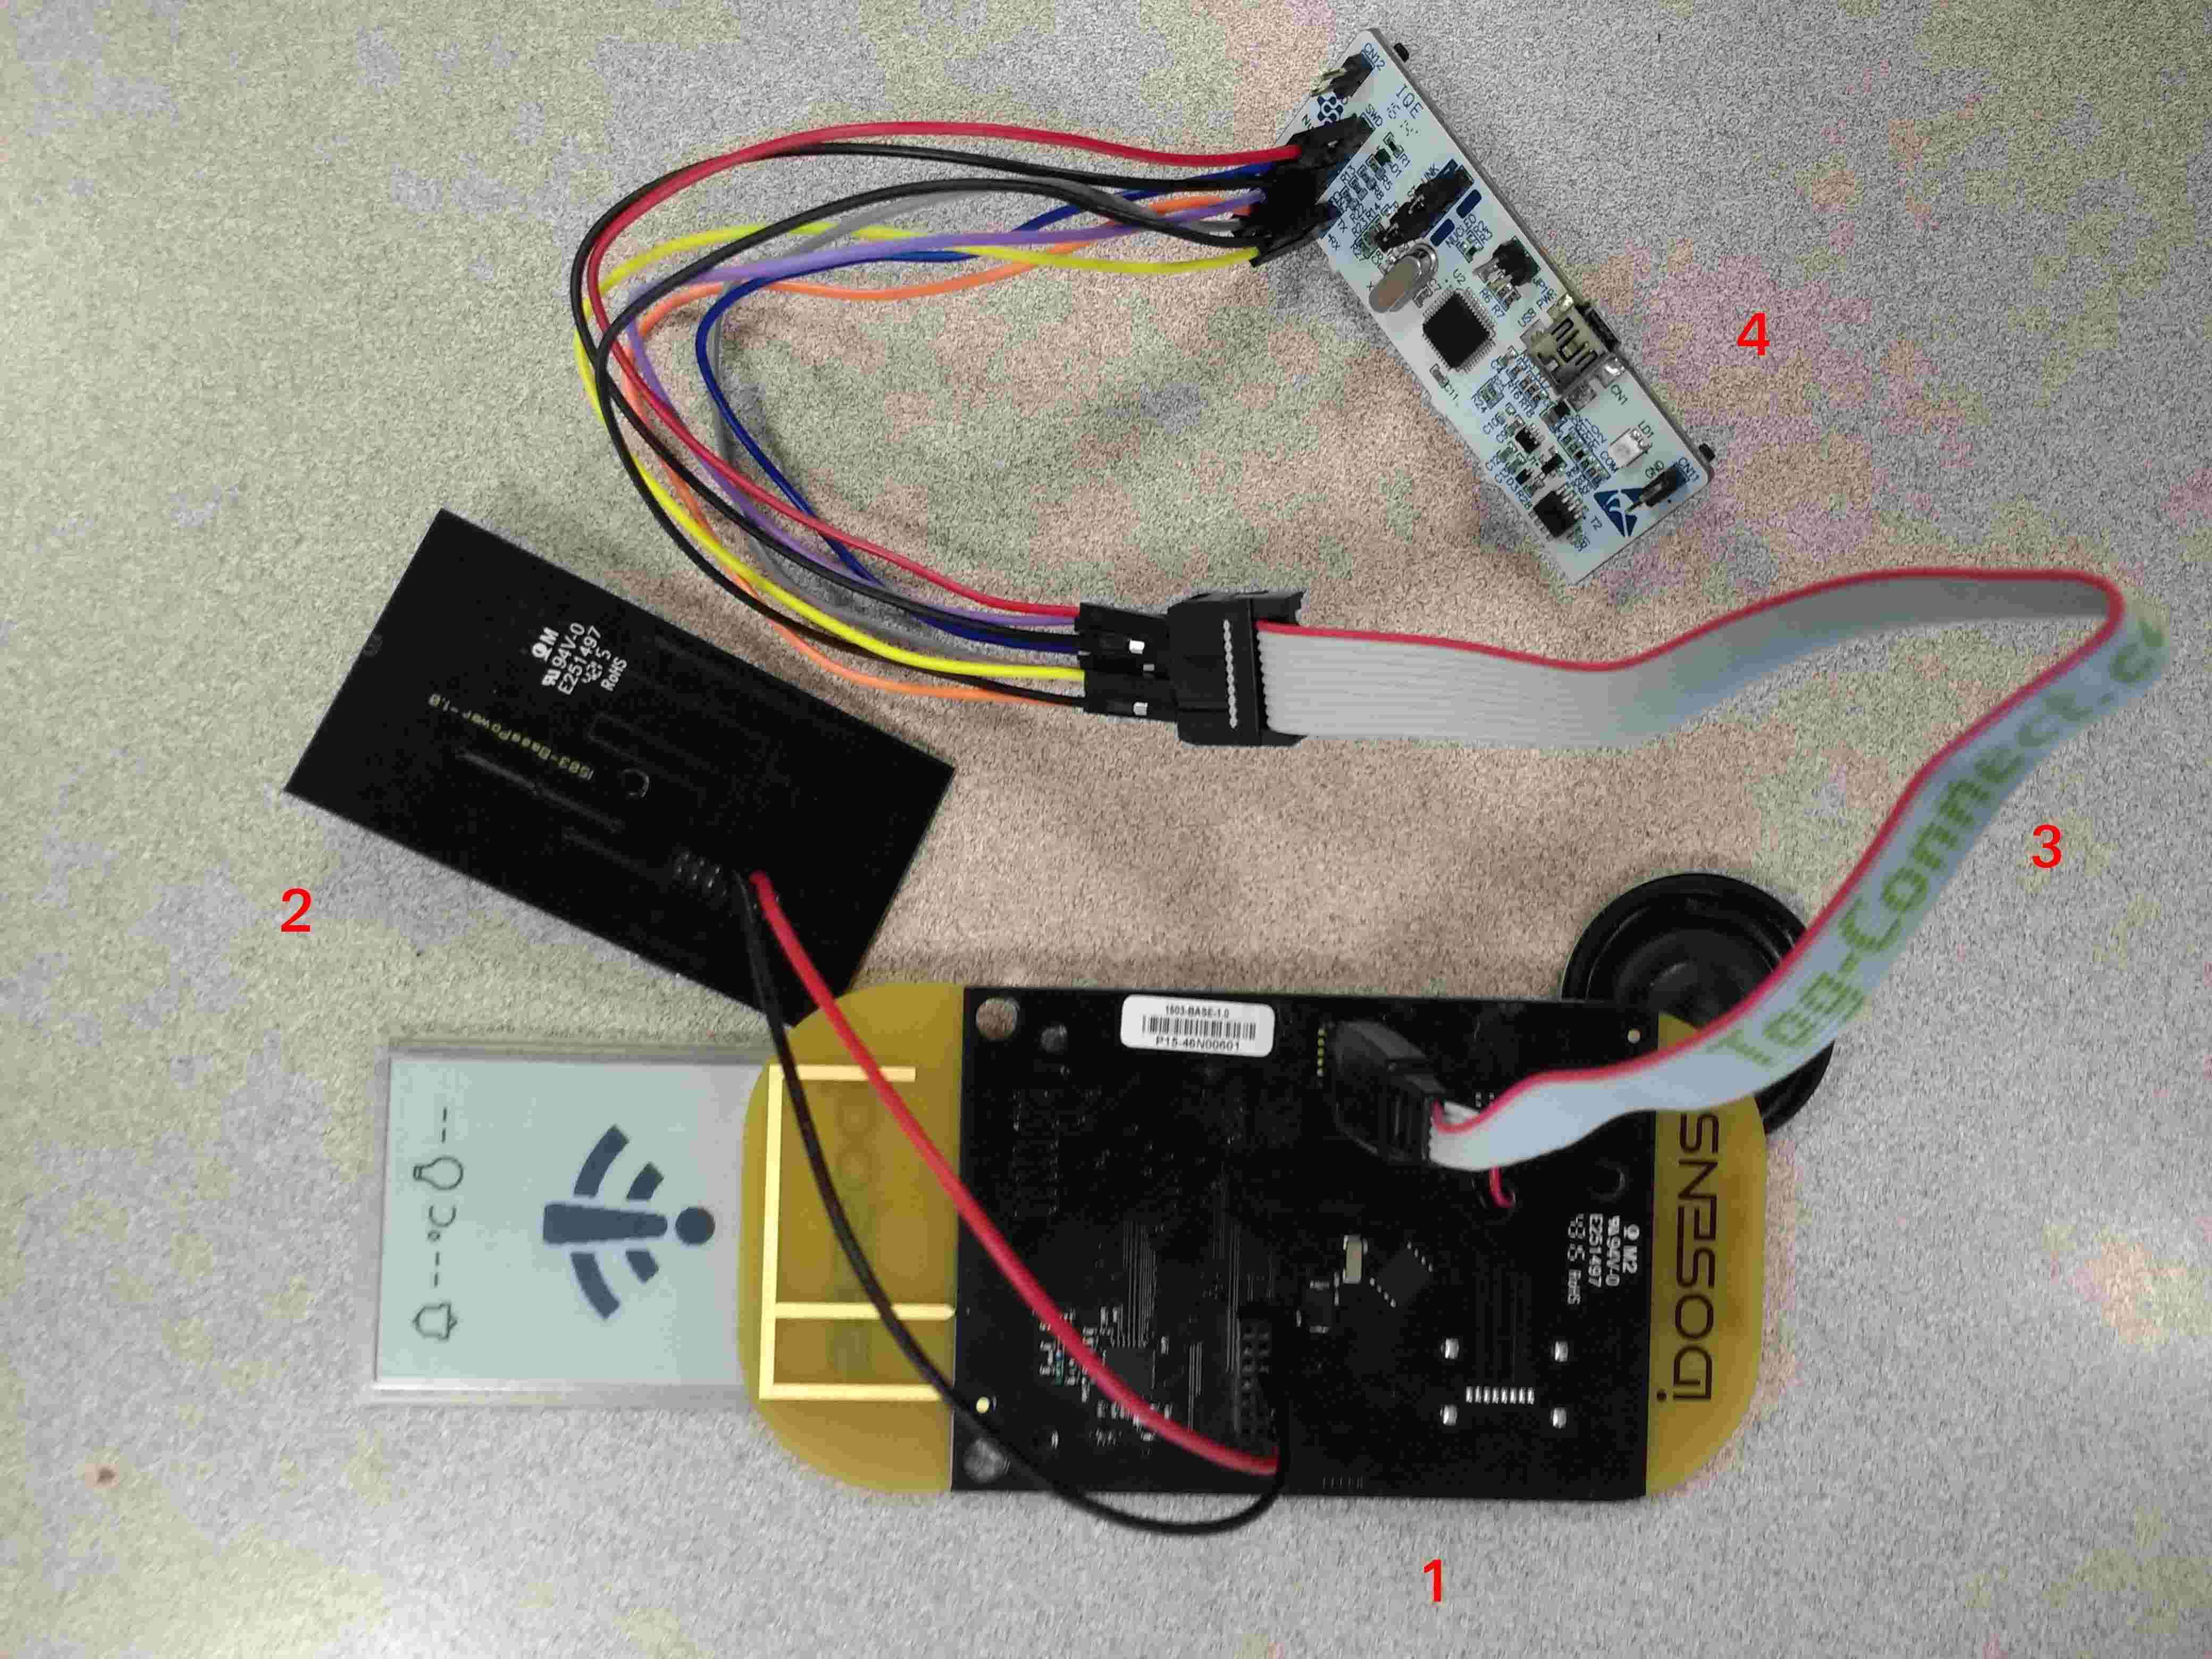
\includegraphics[keepaspectratio=true,scale=0.1]{idosens_numerote.jpg}
\label{visina8}
\end{center}\end{figure}

\begin{itemize}
    \item 1  Base
    \item{2} base power
    \item 3 Tag-connect
    \item 4 ST-LINK
\end{itemize}

\subsection{ST-LINK}
Ce débugueur/flasheur ST-LINK a été prélevé sur une carte nucleo :

\begin{figure}[H]
\begin{center}
\advance\leftskip-3cm
\advance\rightskip-3cm
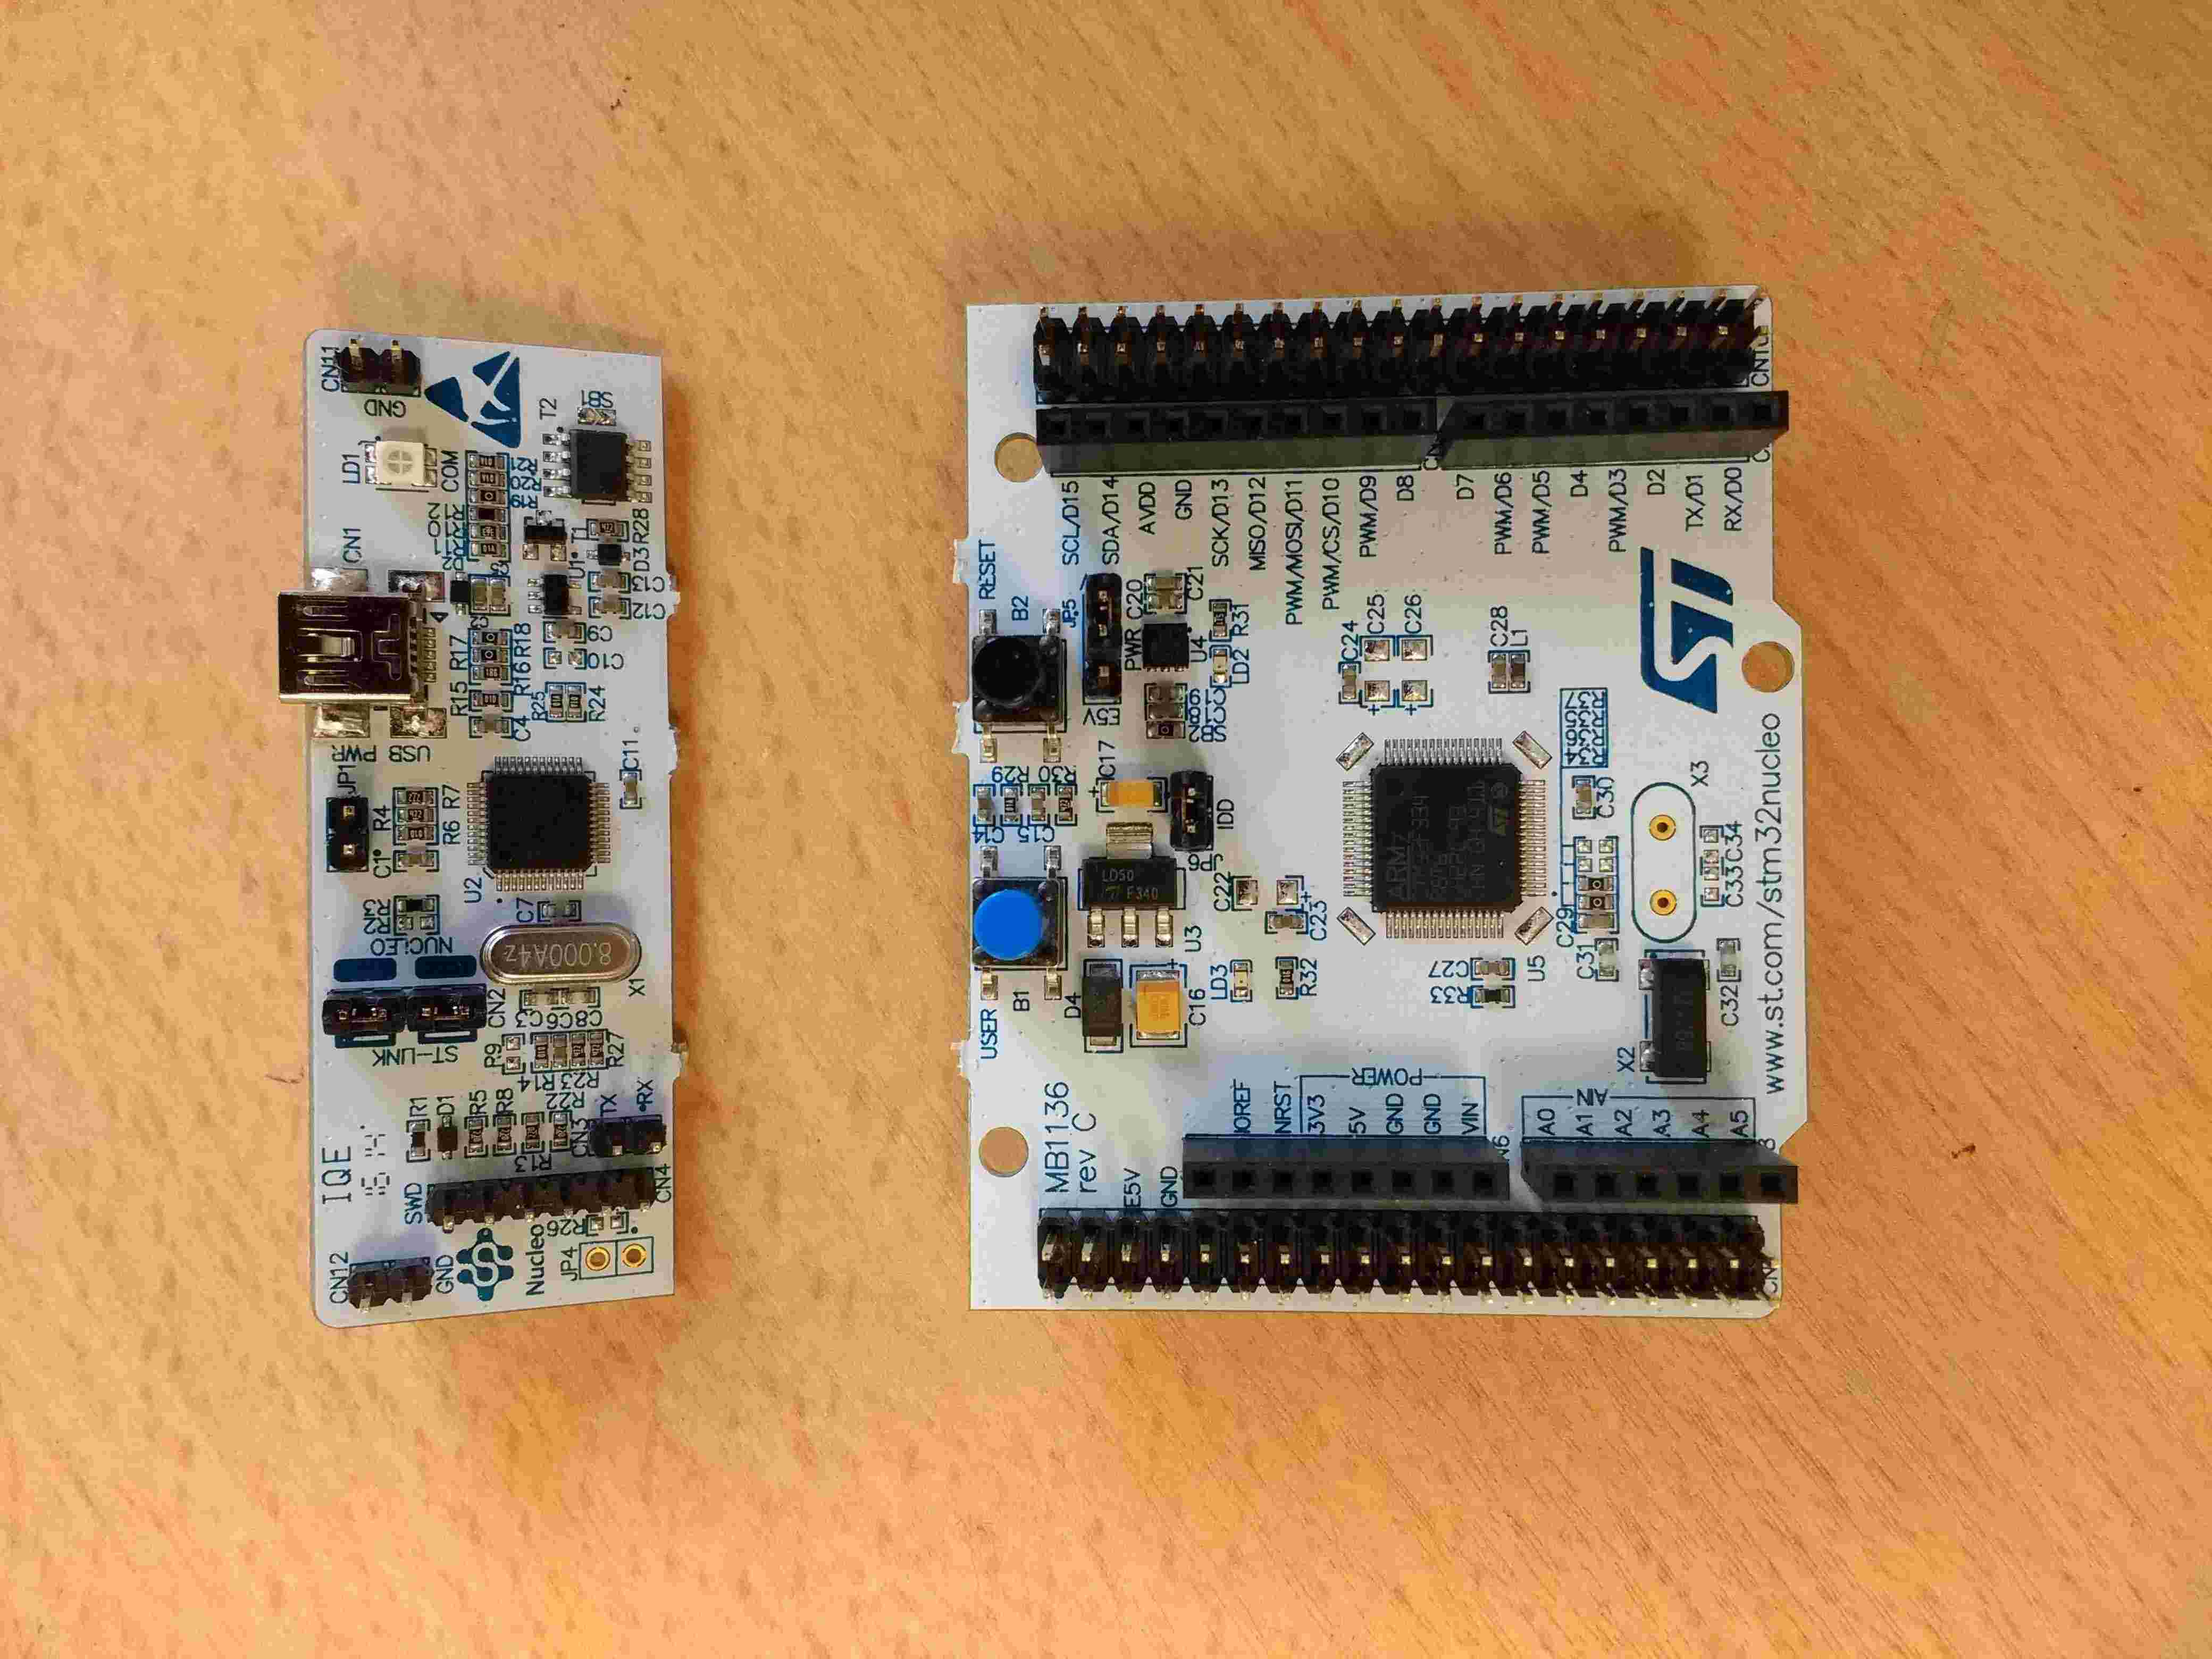
\includegraphics[keepaspectratio=true,scale=0.1]{nucleo_debug.jpg}
\label{visina8}
\end{center}\end{figure}

\subsection{Connexion base power}

\begin{figure}[H]
\begin{center}
\advance\leftskip-3cm
\advance\rightskip-3cm
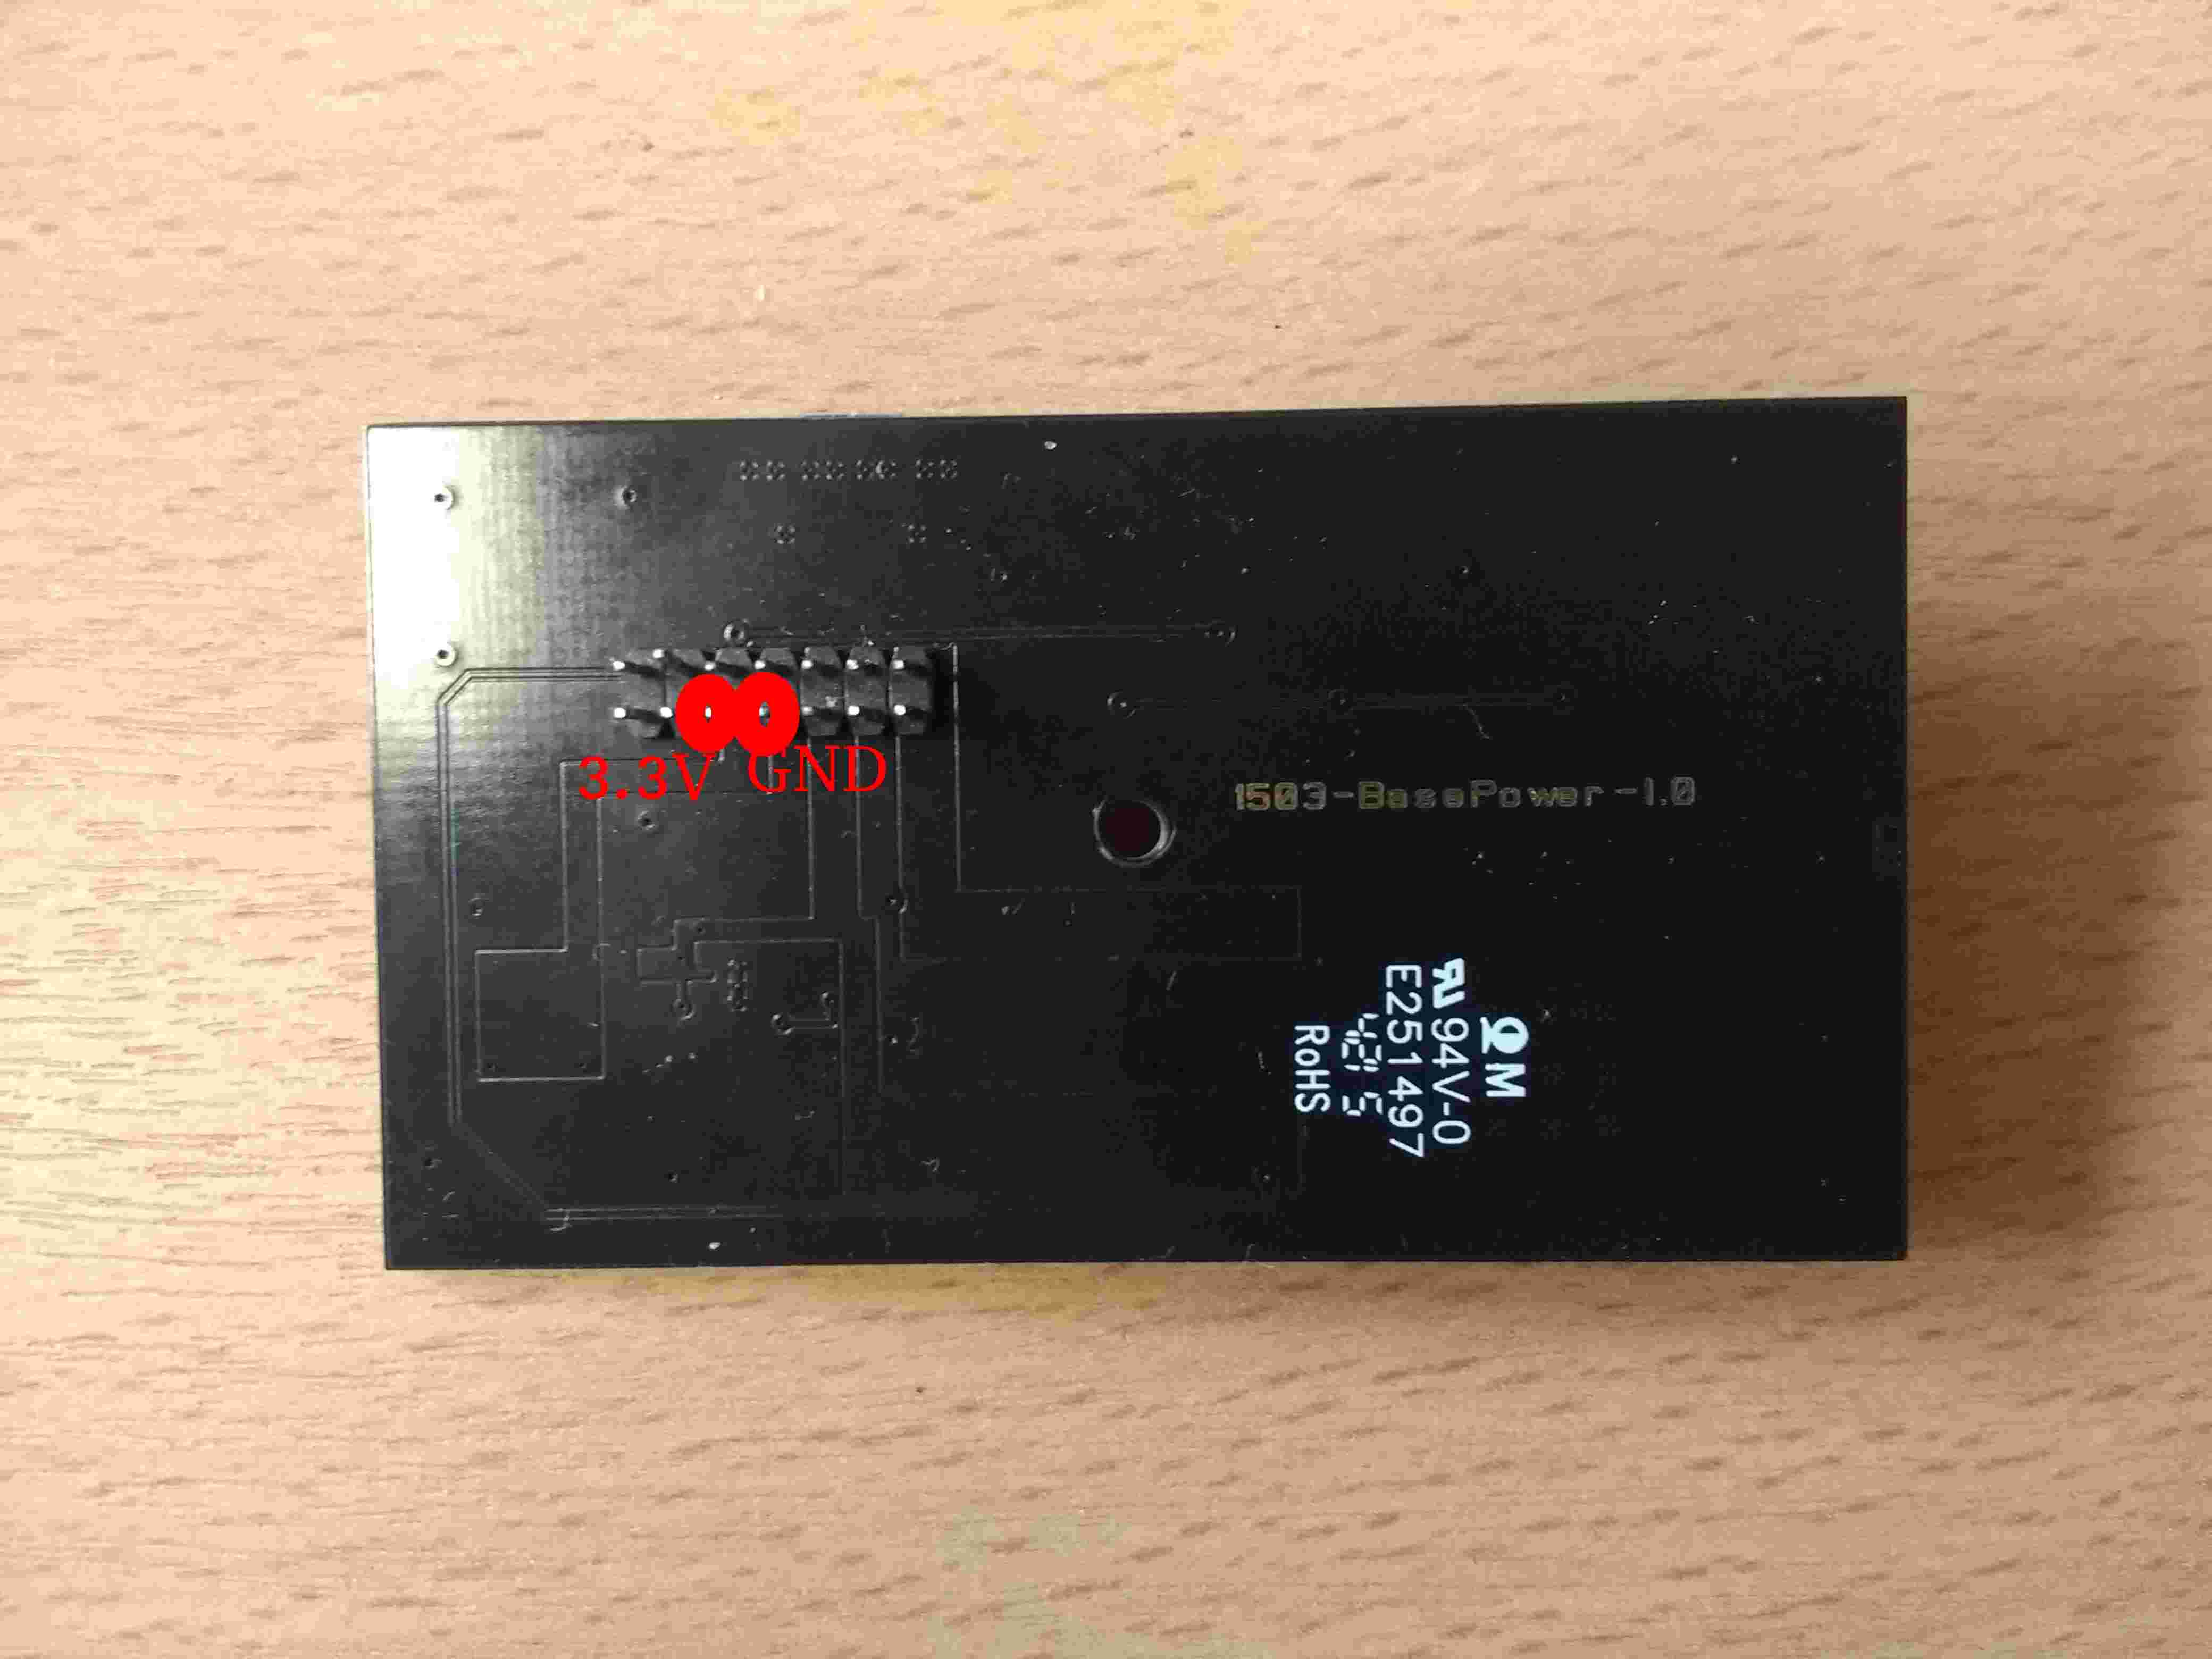
\includegraphics[keepaspectratio=true,scale=0.1]{base_power.jpg}
\label{visina8}
\end{center}\end{figure}

\begin{figure}[H]
\begin{center}
\advance\leftskip-3cm
\advance\rightskip-3cm
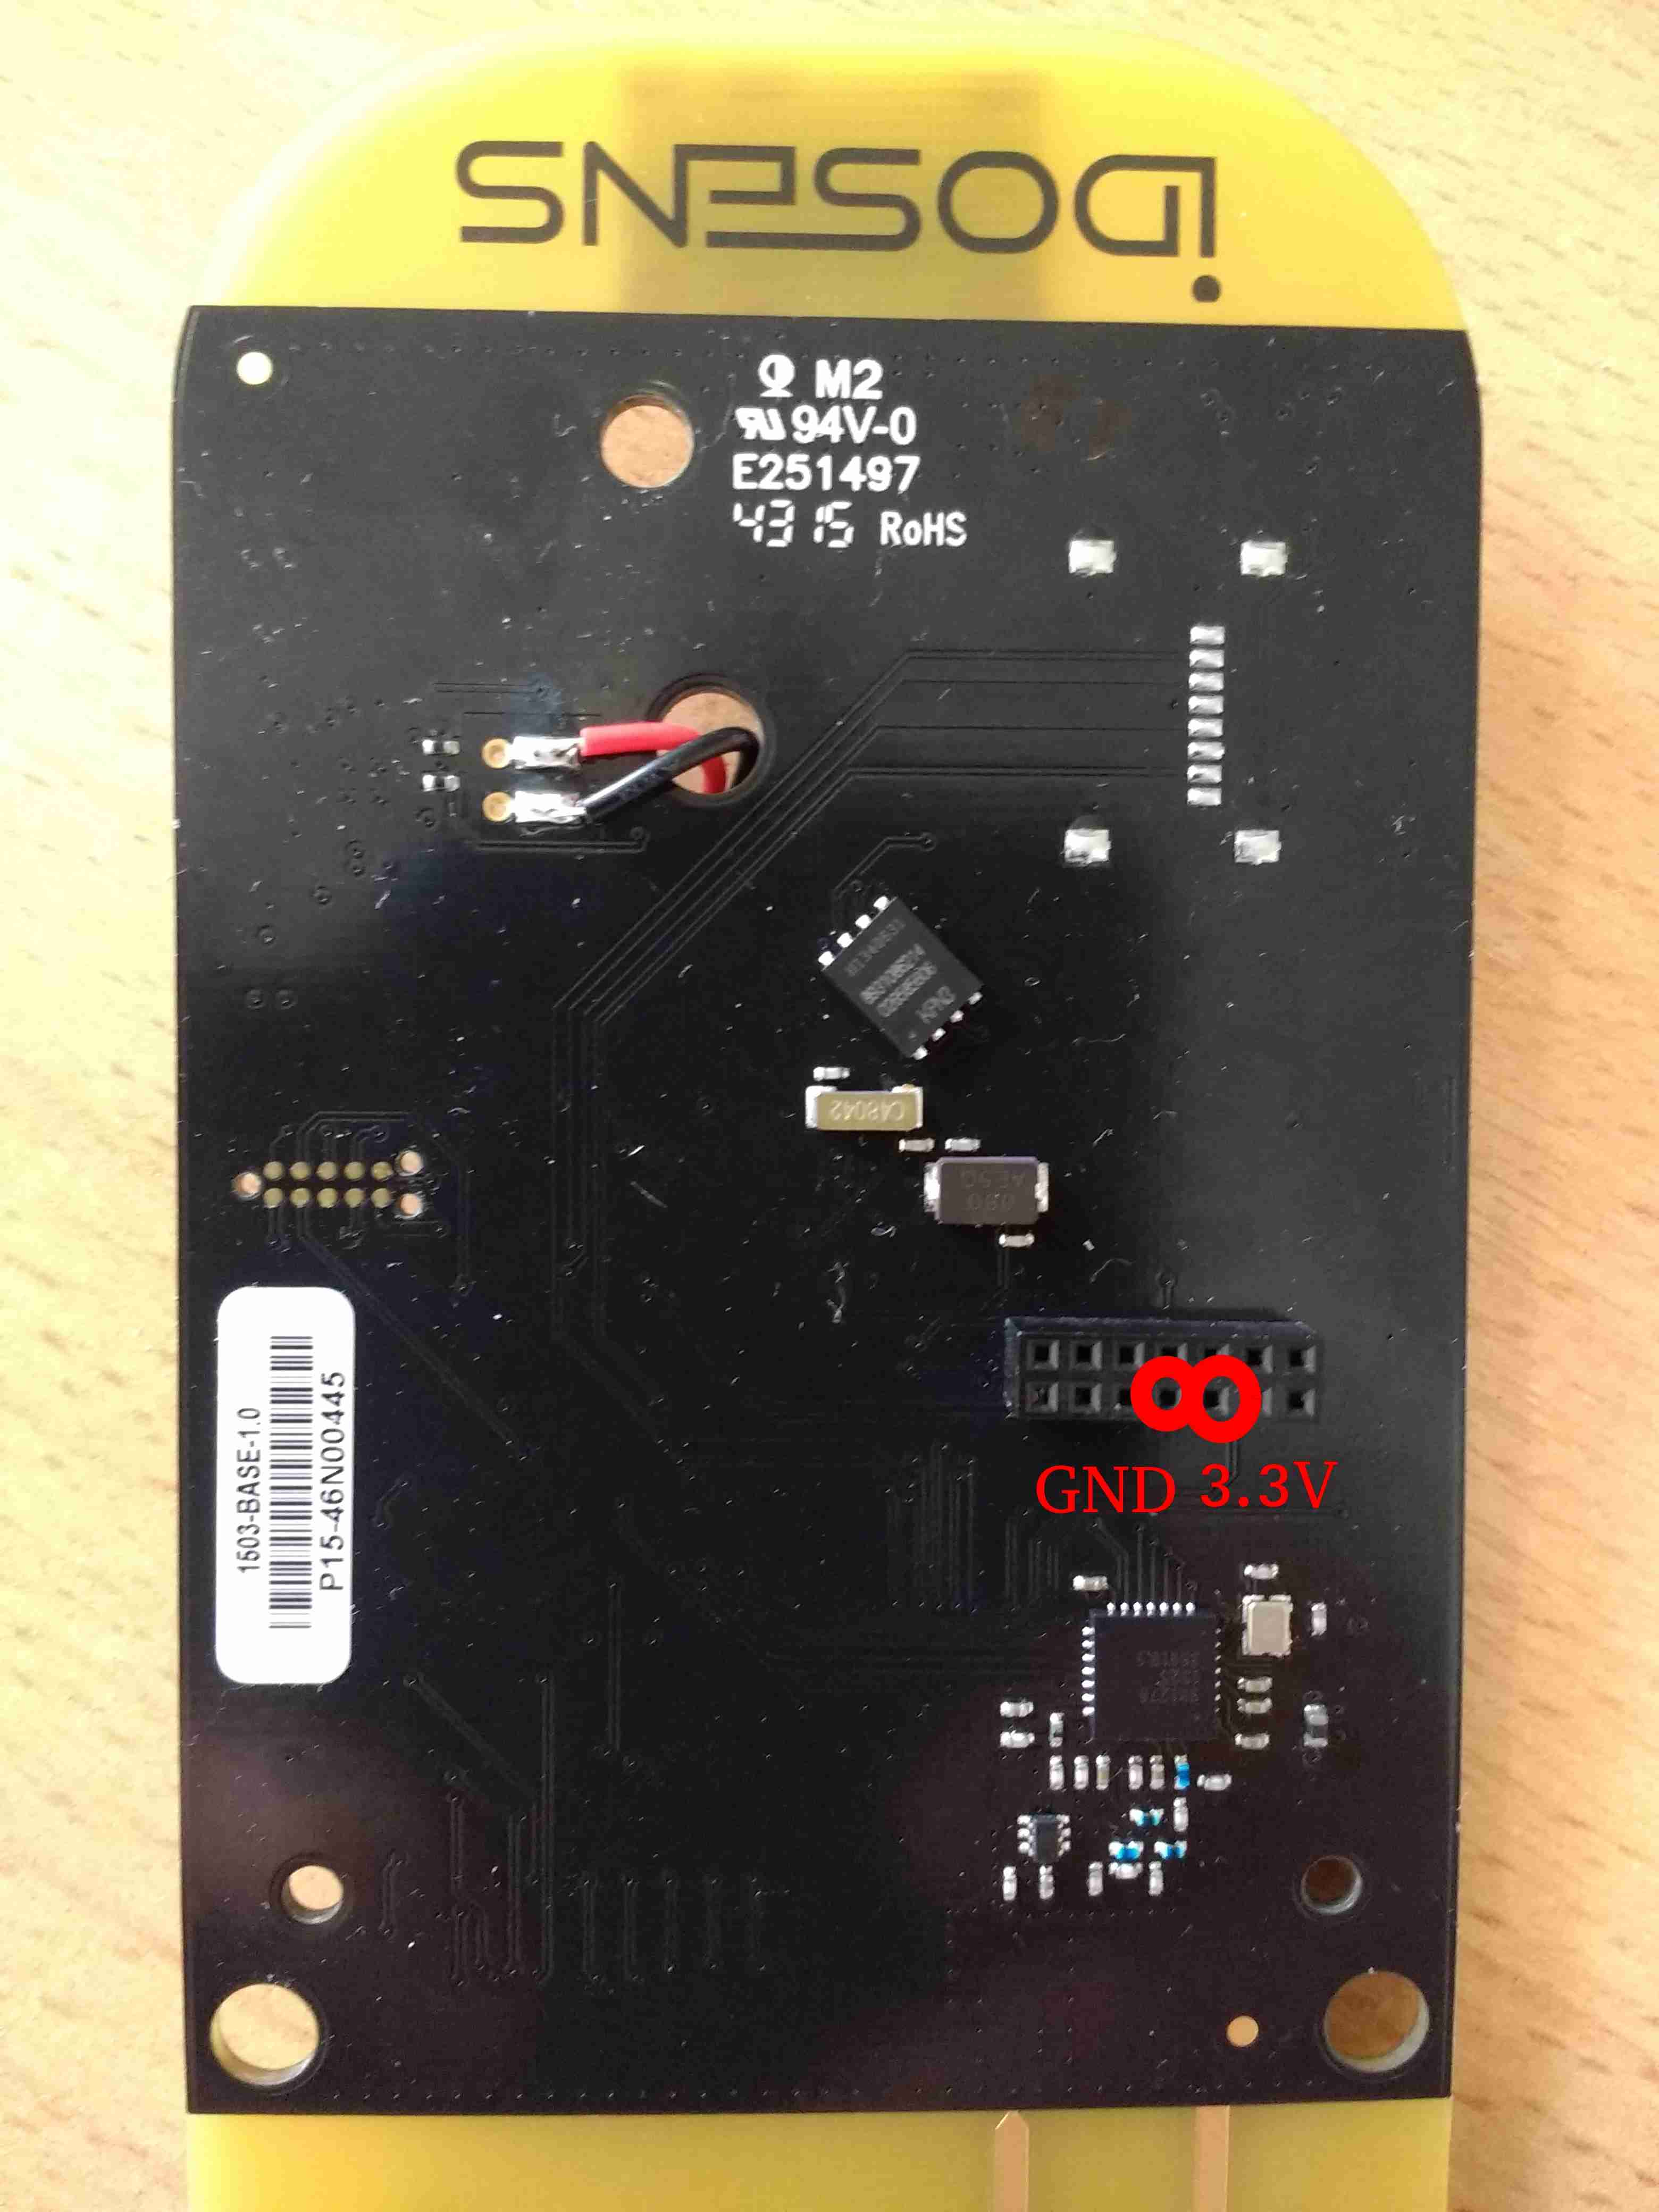
\includegraphics[keepaspectratio=true,scale=0.1]{branchement_basepower2.jpg}
\label{visina8}
\end{center}\end{figure}



\subsection {Connexion ST-LINK-Tag-connect}

Connectez le Tag-connect au nucleo selon ce tableau et selon les schémas des connecteurs :

\begin{figure}[H]
\begin{center}
\advance\leftskip-3cm
\advance\rightskip-3cm
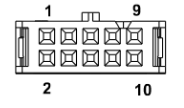
\includegraphics[keepaspectratio=true,scale=0.8]{tag_connectpinout.png}
\label{visina8}
\end{center}\end{figure}

\begin{figure}[H]
\begin{center}
\advance\leftskip-3cm
\advance\rightskip-3cm
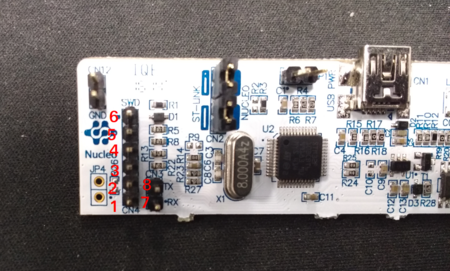
\includegraphics[keepaspectratio=true,scale=0.5]{Nucleo_pins.png}
\label{visina8}
\end{center}\end{figure}

\begin{center}
 \begin{tabular}{||c | c | c ||} 
 \hline
 Pin Nucleo  & Pin Tag-Connect \\ [0.8ex] 
 \hline\hline
   1 Vcc  & 6 VDD TARGET  \\ 
 \hline
    2 SWDIO & 3 SWDIO \\
 \hline
   3 Gnd & 4 GND \\
 \hline
   4 SWCLK &   5 SWCLK\\
 \hline
  X  & X \\ [1ex] 
 \hline
  6 SWO   &  1 SWO\\ [1ex]
 \hline
  7 Tx    & 7 Rx \\ [1ex] 
 \hline
  X  & X \\ [1ex] 
 \hline
  9 Rx &  8 Tx \\ [1ex] 
 \hline
 10 NRST  & 2 NRST\\ [1ex] 
 \hline
\end{tabular}
\end{center}



\section{installation logiciels et configuration du PC}
L'exemple est fait avec ubuntu 16.04
\subsection{Déverouiller ports USB}




ajoutez un fichier 50-myusb.rules dans 

\begin{minted}{bash}
/etc/udev/rules.d

\end{minted}
contenant 

\begin{minted}{bash}
ACTION=="add", KERNEL=="ttyACM[0-9]*", ATTRS{idVendor}=="0483",
ATTRS{idProduct}=="374b", MODE="0666"

\end{minted}

avec idProduct et idVendor à renseigner en fonction du votre produit. On les trouve avec le programme

\begin{minted}{bash}
lsusb

\end{minted}
Redémarrez le PC.

\subsection{Installer pyserial pour communiquer avec la carte}

\begin{minted}{bash}
sudo apt-get install python3-pip
python3 -m pip install pyserial
\end{minted}

\subsection{Installer openocd pour flasher la carte}

\begin{minted}{bash}
sudo apt-get install openocd

\end{minted}


\section{Compiler et utiliser riot}

\subsection{Installer le compilateur gcc-arm-embedded pour générer du code pour la carte}

\begin{minted}{bash}
sudo add-apt-repository ppa:team-gcc-arm-embedded/ppa
sudo apt-get update
sudo apt-get install gcc-arm-embedded

\end{minted}





Téléchargez le code à : \url{https://github.com/CampusIoT/RIOT}\\
Dans un terminal, allez dans 

\begin{minted}{bash}
 extractionPath/RIOT/tests/driver_sx127x/
\end{minted}



Pour lancer la compilation et flasher la carte :
\begin{minted}{bash}
make BOARD=idosens_base flash term
\end{minted}

\section{Ping-Pong idosens}

Avec l'exemple flashé ci-dessus, on peut faire communiquer 2 idosens. Pour cela, le mieux est de connecter un idosens par PC. Une fois l'os flashé, entrez les commandes suivantes :

\begin{itemize}
    \item idosens émetteur
    \begin{figure}[H]
    \begin{center}
    \advance\leftskip-3cm
    \advance\rightskip-3cm
    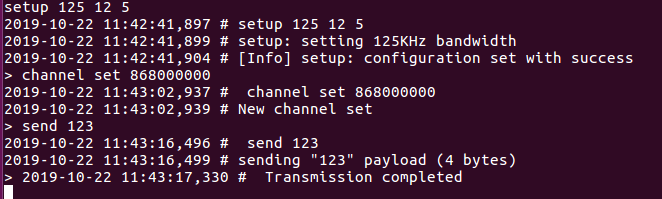
\includegraphics[keepaspectratio=true,scale=0.5]{ping_pong_idosens_sending.png}
    \label{visina8}
    \end{center}\end{figure}
    
    \item idosens récepteur
    \begin{figure}[H]
    \begin{center}
    \advance\leftskip-3cm
    \advance\rightskip-3cm
    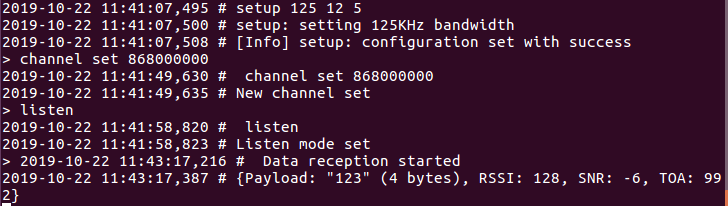
\includegraphics[keepaspectratio=true,scale=0.5]{ping_pong_idosens_receiving.png}
    \label{visina8}
    \end{center}\end{figure}
    
\end{itemize}


\end{document}
